\documentclass{article}

\usepackage[fleqn]{amsmath}
\usepackage{amssymb}
\usepackage{hyperref}
\usepackage{url}
\usepackage{graphicx}
\usepackage{geometry}
\usepackage[italian]{babel}
\usepackage{enumitem}
\usepackage{parskip}
\usepackage{chemfig}
\usepackage{pdfpages}
\usepackage{xcolor}
\usepackage{tikz}
\usepackage{fancybox}
\usepackage{makecell}
\usepackage{soul}

\geometry{
    a4paper,
    total={170mm, 257mm},
    left=20mm,
    top=20mm
}

\hypersetup{
    colorlinks=true,
    linkcolor=black,
    urlcolor=blue,
    pdftitle={Chimica}
}

% === COMMANDS ===
\newcommand{\figbox}[1]{
    \begin{figure*}[h!]
        \begin{center}
            \fbox{#1}
        \end{center}
    \end{figure*}
}

\newcommand*\circled[1]{\tikz[baseline=(char.base)]{
            \node[shape=circle,draw,inner sep=1.1pt] (char) {#1};}
}
\newcommand\angstrom{\mbox{\normalfont\AA}}
\newcommand\namebond[4][5pt]{\chemmove{\path(#2)--(#3)node[midway,sloped,yshift=#1]{#4};}}
\newcommand\arcbetweennodes[3]{
    \pgfmathanglebetweenpoints{\pgfpointanchor{#1}{center}}{\pgfpointanchor{#2}{center}}
    \let#3\pgfmathresult
}
\newcommand\arclabel[8][stealth-stealth,shorten <=1pt,shorten >=1pt]{
    \chemmove{
        \arcbetweennodes{#4}{#3}\anglestart \arcbetweennodes{#4}{#5}\angleend
        \draw[#1]([shift=(\anglestart:#2)]#4)arc(\anglestart:\angleend:#2);
        \pgfmathparse{(\anglestart+\angleend)/2}\let\anglestart\pgfmathresult
        \node[shift=(\anglestart:#2+1pt)#4,anchor=\anglestart+180,rotate=\anglestart#7,
        inner sep=0pt,outer sep=#8]at(#4){#6};
    }
}

% === TEXT ===
\title{\textbf{Chimica \\ Passerella 2023-24}}
\author{Matteo Frongillo}

\begin{document}

\maketitle
\tableofcontents

\begin{center}
    \begin{flushleft}
        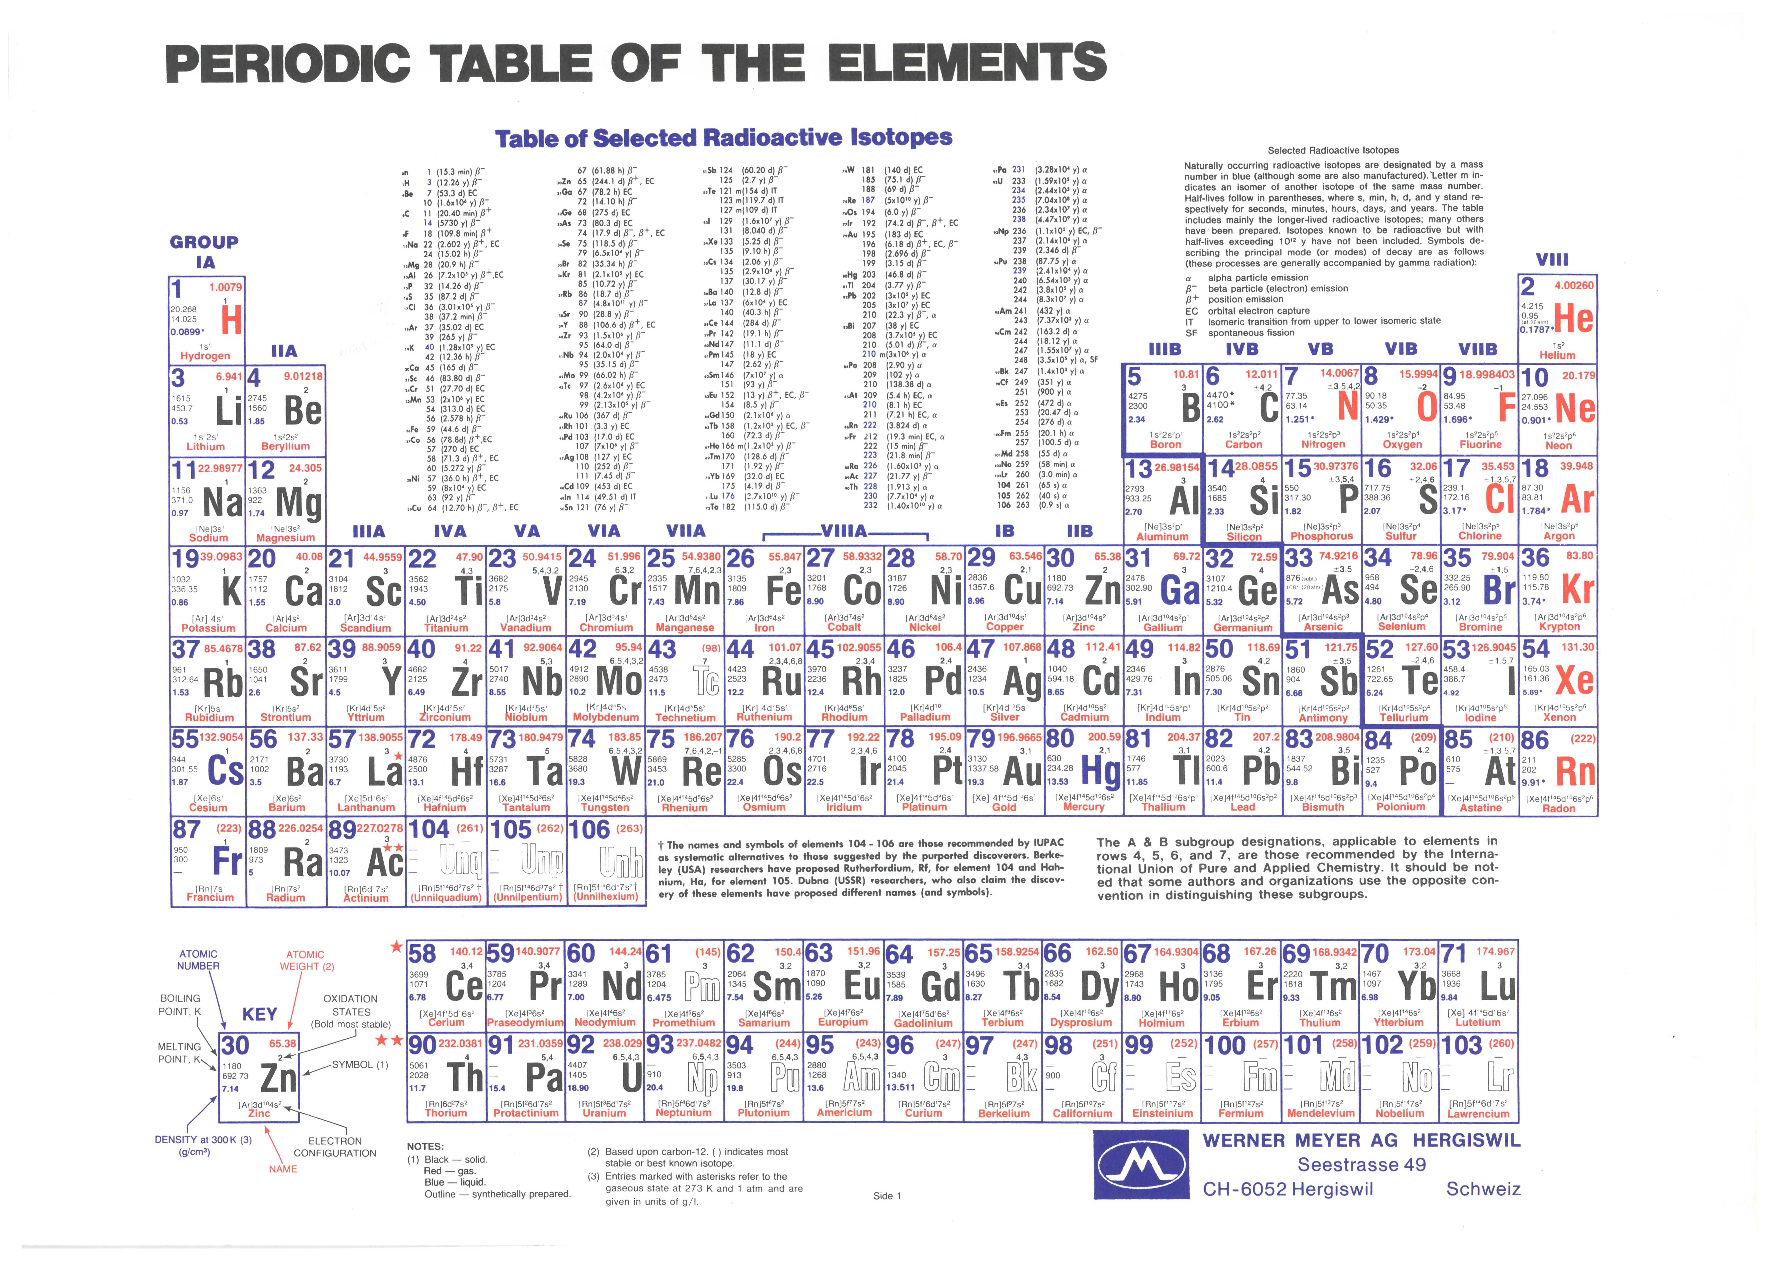
\includepdf[pages={1,2}, nup=1x2, scale=0.8, pagecommand=\section{Tavola periodica}]
        {periodic_table.pdf}
    \end{flushleft}
\end{center}

\pagebreak

\subsection{Organizzazione della tavola periodica}
I \textbf{gruppi} della tavola periodica vengono oraganizzati nella seguente maniera:
\begin{enumerate}[label=\textbf{\Roman*}]
    \item $\rightarrow$ \textbf{metalli alcalini}, formano con l'ossigeno composti alcalini solubili in acqua;
    \item $\rightarrow$ \textbf{metalli alcalino-terrosi,} formano con l'ossigeno composti alcalini non
        sempre solubili in acqua;
    \item $\rightarrow$ \textbf{alogeni}, reagiscono facilmente con i metalli dando composti solidi chiamati sali;
    \item $\rightarrow$ \textbf{gas nobili}, gas poco reattivi.
\end{enumerate}
\vspace{.5cm}

I \textbf{metalli} sono solidi a temperatura ambiente, lucenti, buoni conduttori di elettricità
e calore, duttili e malleabili. Pochi si trovano in natura allo stato puro:
formano composti con non metalli, raramente con altri metalli.
\\ \\
I \textbf{non metalli} hanno proprietà variabili: a temperatura ambiente alcuni sono solidi,
altri liquidi, altri aeriformi, opachi, pessimi conduttori di calore ed elettricità.
Molti si trovano in natura allo stato puro, tutti possono però formare composti sia con metalli
sia con altri non metalli.
\\ \\
I \textbf{semimetalli} hanno proprietà intermedie tra quelle dei metalli e quelle dei non metalli.
\pagebreak

\section{Sostanze pure e miscele}

\subsection{Tipi di trasformazioni}
Esistono tre principali categorie di trasformazioni:
\begin{enumerate}[label=\textbf{\arabic*.}]
    \item \textbf{Trasformazione fisica}\\
        È una trasformazione \underline{reversibile} che non cambia la natura delle sostanze
        coinvolte ma ne modifica l'apparenza \\
        Esempio: la dissoluzione dello zucchero in acqua è una trasformazione fisica, poiché
        lo zucchero rimane tale una volta dissolto nell'acqua, ed essa è possibile invertirla
        tramite le apposite \hyperlink{tecniche di separazione}{\color{blue}{\underline{\textbf{tecniche di separazione}}}}.
    \item \textbf{Reazione chimica}\\
        È un processo attraverso il quale le sostanze modificano la loro identità chimica,
        si trasformano cioè in sostanze differenti \\
        Esempio: la cottura di un uovo è una reazione chimica poiché una volta cotto, esso non
        potrà più tornare allo stato liquido iniziale. Inoltre durante il processo di trasformazione
        si creano nuovi elementi, ad esempio l'odore dell'uovo cotto.
    \item \textbf{Reazione nucleare}\\
        È un processo che riguarda il nucleo di un atomo di uno specifico elemento chimico,
        che viene convertito in un altro a diverso numero atomico coinvolgendo le forze nucleari.
        Esso è suddiviso in due sottocategorie:
        \begin{itemize}
            \item \textbf{Fissione nucleare}: è una reazione nucleare in cui il nucleo più pesante
            decade in atomi di numero atomico inferiore, con emissione di una grande quantità
            di energia e radioattività\\
            Esempio: Bombardamento dell'uranio-235 o del plutonio-239
            \item \textbf{Fusione nucleare}: è una reazione nucleare nella quale i nuclei di due o più
            atomi si uniscono tra loro formando il nucleo di un nuovo elemento chimico.\\
            Esempio: una stella comprime l'idrogeno tramite la sua elevata forza di gravità
            facendolo fondere con altri atomi di idrogeno, formando un atomo di elio.
        \end{itemize}
        
\end{enumerate}

\subsection{Stati di aggregazione}
Gli stati di aggregazione della materia sono gli stati che convenzionalmente può assumere la
materia a seconda delle sue proprietà meccaniche.\\
Gli stati che la materia può assumere sono:
\begin{enumerate}
    \item \textbf{Solido}: La materia ha un volume e una forma propria;
    \item \textbf{Liquido}: La materia ha un volume proprio, ma acquisisce la forma del
        recipiente che la contiene;
    \item \textbf{Gassoso}: La materia non ha né volume né forma propria, ma si espande fino
        a occupare tutto lo spazio disponibile;
    \item \hyperlink{ioni}{\color{blue}{\underline{\textbf{Plasmatico}}}}:
    La materia ionizzata non ha né volume né forma propria, ma si espande fino
    a occupare tutto lo spazio disponibile;
\end{enumerate}

\subsection{Transizione di fase}
La transizione di fase, o passaggio di stato, indica la trasformazione di un sistema termodinamico
da uno stato di aggregazione ad un altro. Durante questa trasformazione, si registra una
variazione dell'entalpia, che quantifica il calore scambiato con l'ambiente a seguito del
cambiamento di stato.

\vspace{-.5cm}
\begin{figure}[h]
    \begin{center}
        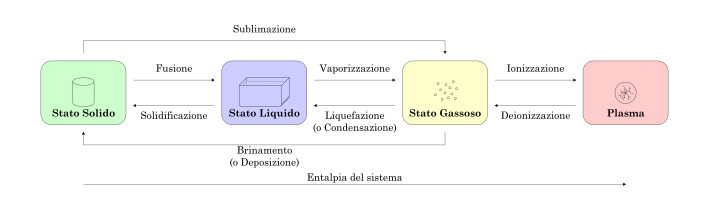
\includegraphics[width=1\textwidth]{Fisica_materia_passaggi_stato_1_it.png}
    \end{center}
\end{figure}

\subsection{La suddivisione della materia}
La materia può essere suddivisa secondo criteri macroscopici:
\begin{center}
    \begin{tikzpicture}[
        level 1/.style = {sibling distance = 5cm},
        level 2/.style = {sibling distance = 2.75cm}
    ]
    \node {\Ovalbox{\large{\textbf{Materia}}}}
        child {
            node {\ovalbox{
                    \begin{minipage}{.11\textwidth}
                        \centering Materia Eterogenea
                    \end{minipage}
                }
            }
        }
        child {
            node {\ovalbox{
                    \begin{minipage}{.10\textwidth}
                        \centering Materia Omogenea
                    \end{minipage}
                }
            }
            child {
                node {\ovalbox{
                        \begin{minipage}{.10\textwidth}
                            \centering Miscuglio Omogeneo
                        \end{minipage}
                    }
                }
            }
            child {
                node {\ovalbox{
                        \begin{minipage}{.08\textwidth}
                            \centering Sostanza pura
                        \end{minipage}
                    }
                }
                child {
                    node {\ovalbox{Composti}}
                }
                child {
                    node {\ovalbox{Elementi}}
                }
            }
        };
    \end{tikzpicture}
\end{center}

\subsection{Le soluzioni (miscugli omogenei)}
Una \textbf{soluzione} è una miscela omogenea formata da due o più sostanze, che presenta
le stesse proprietà in ogni sua parte.

\subsubsection{Solvente e soluto}
Nelle soluzioni viene denominato \textbf{\underline{solvente}} il componente presente in maggior
quantità e \textbf{\underline{soluto}} qualsiasi altra sostanza.\\
La \textbf{\underline{solubilità}} rappresenta la concentrazione massima di un soluto in un certo 
solvente a temperatura costante: la soluzione viene detta \underline{satura}.\\
Quando tentiamo di sciogliere in un solvente una sostanza in quantità maggiore di quella data 
dalla sua solubilità, una parte si scioglie e una parte precipita, depositandosi come \textbf{corpo di fondo}.

\subsubsection{La concentrazione}
La \textbf{\underline{concentrazione}} è definita come rapporto tra la quantità di soluto 
e quantità di soluzione o solvente. \\
Per esprimere la concentrazione di una soluzione sono possibili tre tipi di composizioni percentuali:
\begin{equation*}
    \text{Percentuale in massa: }
    \%\frac{m}{m} = \frac{massa_{soluto}}{massa_{soluzione}}\cdot100
\end{equation*}\\
\begin{equation*}
    \text{Percentuale in volume: }
    \%\frac{V}{V} = \frac{V_{soluto}}{V_{soluzione}}\cdot100
\end{equation*}\\
\begin{equation*}
    \text{Percentuale in massa su volume: }
    \%\frac{m}{V} = \frac{m_{soluto}}{V_{soluzione}}\cdot100
\end{equation*}\\
\begin{equation*}
    \text{Concentrazione:}
\end{equation*} 
\begin{equation*}
    C\ [\%\frac{m}{m}] = \frac{m_{soluto}}{m_{soluzione}\cdot\rho_{soluzione}}
\end{equation*}\\
\begin{equation*}
    C\ [\%\frac{V}{V}] = \frac{V_{soluto}}{V_{soluzione}\cdot\rho_{soluzione}}
\end{equation*}\\
\begin{equation*}
    C\ [\%\frac{m}{V}] = \frac{m_{soluto}}{V_{soluzione}\cdot\rho_{soluzione}}
\end{equation*}\\
\begin{equation*}
    \text{Proporzionalità: } C_1V_1=C_2V_2 \Rightarrow C_2=\frac{C_2V_2}{V_1}
\end{equation*}

\subsubsection{La diluizione}
La diluizione è un'operazione che comporta \underline{l'aggiunta di solvente} a una soluzione
in modo tale da portare il valore della concentrazione della soluzione da un valore iniziale
$M_1$ ad un valore finale $M_2$ inferiore a quello iniziale.
Durante la diluizione il volume della soluzione pertanto aumenta, la concentrazione
della soluzione diminuisce e il numero di moli $n$ rimane invariato, dunque $n_i=n_f$
\begin{equation*}
    M_1 \cdot V_1 \cdot \text{\st{$n_i$}} = M_2 \cdot V_2 \cdot \text{\st{$n_f$}}
    \Rightarrow  M_1 \cdot V_1 = M_2 \cdot V_2
\end{equation*}

\subsubsection{La solubilità dei gas}
La solubilità dei gas nei liquidi è influenzata dalla pressione e dalla temperatura del fluido.
Al contrario di quello che avviene per la maggior parte dei solidi, la solubilità dei gas
\underline{diminuisce all'aumentare della temperatura}, ma \underline{aumenta all'aumentare della pressione} \\

\fbox{
    \begin{minipage}{1\textwidth}
        \textbf{Legge di Henry:}\\
        La quantità di gas che si scioglie in un dato volume di liquido, a una data temperatura, è 
        direttamente proporzionale alla pressione di quello stesso gas presente sopra la superficie del
        liquido.
    \end{minipage}
}


\subsubsection{Effetto Tyndall}
L'effetto Tyndall è un effetto ottico che si osserva quando la luce passa attraverso una miscela
contenente particelle di dimensioni tali da disperdere la luce.
Questo fenomeno è tipico nelle miscele eterogenee, dove le particelle sono abbastanza grandi
per essere visibili. Le soluzioni vere, invece, non mostrano l'effetto Tyndall poiché contengono
particelle molto piccole (0.2 a 2 nm), le quali non sono abbastanza grandi per disperdere la luce.

\subsection{Riassunto}
\begin{itemize}
    \item Le soluzioni sono miscele omogenee di due o più sostanze che costituiscono
        \textbf{sistemi monofasici};
    \item La sostanza in quantità maggiore è detta \textbf{solvente}, mentre quella in quantità
        minore e disciolta nel solvente è detta \textbf{soluto};
    \item La solubilità rappresenta la concentrazione massima di un soluto in un certo solvente
        a temperatura costante: la soluzione viene detta in questo caso satura;
    \item Una soluzione insatua può essere diluita o concentrata;
    \item La grandezza che esprime la composizione di una soluzione è detta \textbf{concentrazione}
        e per esprimerla vi sono i modi $\% \frac{m}{m}$, $\% \frac{V}{V}$ e $\% \frac{m}{V}$;
    \item In generale, più la temperatura dell'acqua è alta, più una sostanza solida si scioglie
        facilmente in essa. Cambiamenti nella pressione non influenzano questo processo di solubilità;
    \item La capacità di un gas di sciogliersi in un liquido diminuisce se la temperatura aumenta,
        ma aumenta se la pressione diventa più alta;
    \item Il modo di distinguere una soluzione da una miscela eterogenea è basato sulle dimensioni
        delle particelle: se il diametro delle particelle è compreso tra 0.2 e 2 nm, la miscela
        è considerata omogenea, come una soluzione. Inoltre esse non mostrano l'effetto Tyndall.
\end{itemize}
\pagebreak

\hypertarget{tecniche di separazione}{}
\section{Le tecniche di separazione}
\subsection{Separazione dei miscugli eterogenei e omogenei}
    Le componenti di un \textbf{miscuglio eterogeneo} possono essere separate con \underline{metodi meccanici}:
        \begin{itemize}
            \item \textbf{Decantazione}: è un processo spontaneo che realizza la separazione di miscugli
                solido-liquidi per mezzo della forza di gravità in base alla densità delle sostanze;
            \item \textbf{Centrifugazione}: inserendo un miscuglio eterogeneo in una centrifuga, esso
                verrà roteato ponendo il fluido a una forza centrifuga, rendendo più rapida la
                sedimentazione della sostanza con densità maggiore; 
            \item \textbf{Filtrazione}: versando un fluido con un materiale sospeso al suo interno attraverso
                un setto poroso, permette di separare il fluido dal materiale.
        \end{itemize}
    Le componenti di un \textbf{miscuglio omogeneo (soluzioni)} possono essere separate con \underline{metodi fisici}:
        \begin{itemize}
            \item \textbf{Distillazione semplice}: questa tecnica sfrutta le volatilità differenti
                tra le sostanze in una miscela per separarle;
            \item \textbf{Cristallizzazione}: viene fatto sciogliere il solido nella minima quantità di
                solvente a caldo, si filtra la soluzione e si fa raffreddare lentamente il filtrato,
                così da avere la sostanza separata sottoforma di cristallo;
            \item \textbf{Estrazione}: per separare due liquidi immiscibili, si sfrutta la loro diversa
                solubilità in un determinato solvente. Il solvente scelto dovrà sciogliere selettivamente
                soltando uno dei due liquidi, permettendo la completa separazione delle fasi;
            \item \textbf{Cromatografia}: sfrutta la diversa affinità dei componenti della miscela
                verso due fasi diverse e permette di separare i componenti sfruttando la solubilità,
                dimensione delle particelle e fenomeni di assorbimento.
            \end{itemize}
    Inoltre, le componenti di un \textbf{miscuglio omogeneo (soluzione)} possono essere separate anche con \underline{metodi chimici}:
        \begin{itemize}
            \item \textbf{Dialisi}: separa i soluti in base alla loro dimensione e alla loro capacità
                di diffondere attraverso una membrana semipermeabile;
            \item \textbf{Precipitazione}: vengono aggiunti reagenti che causano la formazione di un
                solido insolubile (precipitato) da una soluzione, che può essere separato per filtrazione;
        \end{itemize}
\pagebreak

\section{Modello atomico}
\subsection{L'atomo}
    L'atomo è l'unità base della materia, composto da un nucleo centrale e da elettroni che orbitano
    attorno ad esso.
        \subsubsection{Il nucleo atomico}
            Il nucleo di un atomo è formato da protoni e neutroni (ad eccezione dell'isotopo prozio $_1^1$H,
            il cui nucleo è costituito unicamente da un protone). L'unità di misura che indica la dimensione
            degli atomi è l'ångström (Å), il cui valore corrisponde a 0.1 nm o 10$^{-10}$ m.\\
            I \textbf{protoni} ($p^+$) sono particelle subatomiche non elementari dotate di carica elettrica positiva,
            mentre i \textbf{neutroni} ($n^0$) sono particelle subatomiche non elementari con carica elettrica netta pari
            a zero.
        \subsubsection{Gli orbitali atomici}
            Gli orbitali atomici sono regioni definite dello spazio attorno al nucleo di un
            atomo dove la probabilità di trovare un elettrone è massima.\\
            Gli \textbf{elettroni} ($e^-$) sono particelle subatomiche con carica elettrica negativa.
            A differenza dei protoni e dei neutroni, gli elettroni sono particelle elementari.
            Gli elettroni sono responsabili della formazione dei legami chimici tra gli atomi.
\subsection{Il numero atomico e la massa atomica}
    Il numero atomico ($Z$) è il \underline{numero di protoni} presenti in un atomo:
    tutti gli atomi di uno stesso elemento hanno lo stesso numero atomico.
    Il numero atomico corrisponde anche al numero di elettroni.
        \begin{figure}[h]
            \centering \fbox{numero atomico = numero $p^+$}\: \textrightarrow\ $_Z$X
        \end{figure} \\
    Il numero di massa ($A$) è la \underline{somma del numero di protoni e neutroni} presenti
    in un atomo.\\
    {\color{red}Il numero di neutroni varia in base all'isotopo preso in considerazione!}
        \begin{figure}[h]
            \centering \fbox{numero di massa = numero $p^+$ + $n^0$}\: \textrightarrow\ $^A_Z$X
        \end{figure} \\
    Il numero di neutroni è dunque calcolabile sottraendo il numero atomico dal numero di massa.
        \begin{figure}[h]
            \centering \fbox{numero di $n^0$ = $A$ - $Z$}
        \end{figure}

\hypertarget{ioni}{}
\subsection{Gli ioni}
    Gli ioni si formano quando un atomo perde o guadagna uno o più elettroni.
    Questo fenomeno viene chiamato ionizzazione e gli atomi che la subiscono diventano
    particelle cariche.\\
    Gli ioni che acquisiscono elettroni, quindi presentano una carica negativa, sono chiamati
    \textbf{anioni} (X$^{n-}$).\\
    Al contrario, gli atomi che perdono elettroni, quindi presentano
    una carica negativa, sono definiti \textbf{cationi} (X$^{n+}$).\\
    Quando i gas si ionizzano, formano uno stato della materia conosciuto come \textbf{plasma}.

\subsection{Struttura dell'atomo}
\begin{figure*}[h!]
    \begin{center}
        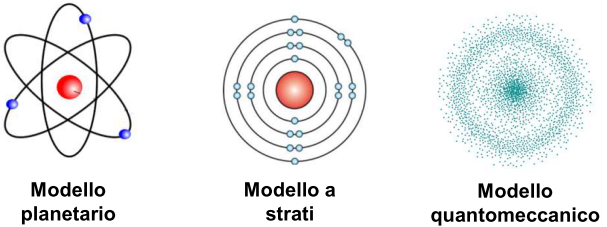
\includegraphics[width=.6\textwidth]{Struttura_atomi.png}
    \end{center}
\end{figure*}

\subsection{Energia di ionizzazione}
L'energia di ionizzazione (EI) è l'energia necessaria per allontanare un elettrone da un atomo o da
uno ione gassoso nel suo stato fondamentale. Gli atomi con più di un elettrone hanno più valori
di energia di ionizzazione, che corrispondono all'allontanamento successivo degli elettroni.\\
L'energia di \underline{prima ionizzazione} aumenta con il numero totale di elettroni di valenza
e aumenta con il numero di orbite.

\subsection{Affinità elettronica}
L'affinità elettronica (AE) è la variazione di energia potenziale [$\frac{kJ}{mol}$] dovuta
all'aggiunta di un elettrone a un atomo o di uno ione gassoso nel suo stato fondamentale.
L'aggiunta di un elettrone a un atomo neutro è quasi sempre un processo \textit{esotermico},
(valori di AE negativi).\\
L'affinità elettronica aumenta con il numero totale di elettroni di valenza e aumenta
con il numero di orbite.

\hypertarget{elettronegatività}{}
\subsection{Elettronegatività}
L'elettronegatività ($E_N$) è la forza intramolecolare tra due atomi.
Essa esprime la capacità di un atomo di attrarre gli elettroni nel legame in cui è convolto.\\
L'elettronegatività aumenta con il numero totale di elettroni di valenza e diminuisce
con il numero di orbite.
\begin{figure*}[h!]
    \centering \includegraphics[width=.75\textwidth]{elettronegatività.png}
\end{figure*}

\pagebreak

\section{Chimica nucleare e radioattività}
\subsection{Gli isotopi}
Un isotopo è un atomo, di un qualunque elemento chimico, che mantiene lo stesso numero atomico ($Z$)
ma differente numero di massa ($A$), di conseguenza differente massa atomica ($M$).
La differenza nel numero di massa è dovuta al \underline{differente numero di neutroni} che possono
essere presenti nel nucleo di atomi aventi lo stesso numero atomico ($Z$).

\hypertarget{massa atomica}{}
\subsection{Massa atomica degli elementi}
La massa atomica di un elemento si calcola dopo aver determinato sperimentalmente la massa dei
singoli isotopi e la percentuale con cui essi sono presenti in natura:\\
\begin{center}
    \fbox{
        \centering $MA=\frac{\%_{\text{isotopo1}}\ \times\ m_{\text{isotopo1}}\ +\ 
            \%_{\text{isotopo2}}\ \times\ m_{\text{isotopo2}}\ +\ \ldots\ +\ 
            \%_{\text{isotopo\ n}}\ \times\ m_{\text{isotopo\ n}}}{100}$ [\text{u}]
    }
\end{center}

\subsection{La radioattività}
Nel nucleo degli atomi è presente una \textbf{forza nucleare forte}, che tiene uniti protoni e neutroni.
La stabilità di un nucleo dipende dal confronto tra le forze elettrostatiche repulsive tra i protoni
e le forze nucleari attrattive tra protoni e neutroni.\\
Al fine di raggiungere una maggiore stabilità, i nuclei \textbf{radionuclidi} (isotopi intabili) vanno
in contro a un \textbf{decadimento radioattivo}. Questo fenomeno si chiama \textbf{radioattivià}.

\subsubsection{\large Decadimento $\alpha$} 
Vengono emessi \textbf{nuclei di elio} ($^4_2$He). \\
Con l'emissione di particelle $\alpha$ il numero di massa ($A$) diminuisce di quattro unità
e il numero atomico ($Z$) di due.
\begin{figure*}[h]
    \begin{center}
        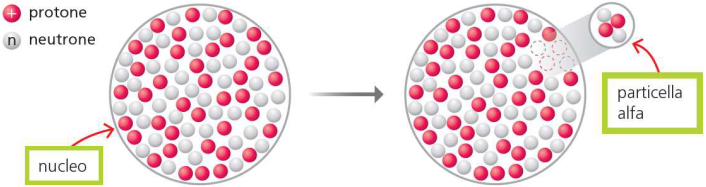
\includegraphics[width=.6\textwidth]{Decadimento_alfa.png}
    \end{center}
\end{figure*}
\begin{center}
    \fbox{
        \centering $^A_Z$X $\rightarrow\, ^{A-4}_{Z-2}$Y + $^4_2$He
    }
\end{center}

\subsubsection{\large Decadimento $\beta^-$}
Quando \underline{un neutrone si trasforma in protone} si ha l'emissione di un elettrone negativo
($e^-$): $n^0 \rightarrow p^++^{\ \: 0}_{-1}e$
\begin{center}
    \fbox{
        \centering $^A_Z$X $\rightarrow ^A_{Z+1}$Y $+^{\ \: 0}_{-1}e$ 
    }
\end{center}

\subsubsection{\large Decadimento $\beta^+$}
Quando \underline{un protone si trasforma in neutrone} si ha l'emissione di un elettrone positivo
($e^+$): $p^+ \rightarrow n^0+^{0}_{1}e$
\begin{center}
    \fbox{
        \centering $^A_Z$X $\rightarrow ^A_{Z-1}$Y $+^{0}_{1}e$ 
    }
\end{center}

\subsubsection{\large Decadimento $\gamma$}
Nel decadimento $\gamma$ vengono emessi \textbf{fotoni a energia elevata} ($^0_0\gamma$).
Con l'emissione di queste particelle il numero di massa e il numero atomico rimangono invariati.
\begin{center}
    \fbox{
        \centering $^0_1e \rightarrow \leftarrow ^{\ \: 0}_{-1}e \ 
        \longrightarrow\ ^0_0\gamma \leftrightsquigarrow\ ^0_0\gamma$ 
    }
\end{center}

\subsection{Tempo di dimezzamento}
Il tempo di dimezzamento ($t_{1/2}$) è il tempo necessario per dimezzare la quantità iniziale
di un radionuclide con il decadimento ed è dato dalla seguente equazione:
\begin{center}
    \fbox{
        \centering $N(t)=N_0\cdot e^{kt}\ \Rightarrow\ t_{1/2}=\frac{\text{ln}2}{k}$
    }
\end{center}

\subsection{Fusione nucleare}
La fusione nucleare è la fusione di due nuclei leggeri in un nucleo più pesate. Essa è resa 
possibile in natura dalle temperature molto elevate e dalle enormi pressioni presenti nei nuclei
delle stelle.
\begin{center}
    \fbox{
        \centering $^3$H + $^2$H\ $\rightarrow\ ^4$He + $^1_0$n
    }
\end{center}
\pagebreak

\section{Reazioni chimiche}
\subsection{Il linguaggio delle formule}
\begin{itemize}
    \item A pedice di ogni simbolo chimico si indica quanti atomi o ioni di un elemento sono presenti
        nella molecola, a condizione che il numero di essi sia maggiore di 1 unità:
    \begin{figure*}[h!]
        \begin{center}
            \fbox{
                {\centering \chemfig{\Charge{-135=\|,135=\|}{O}=[:00]\Charge{45=\|,-45=\|}{O}} \textrightarrow\ O$_2$}
            }
        \end{center}
    \end{figure*}

    \item Quando una sostanza è formata da \underline{ioni}, nella formula si indica solo la
        carica complessiva della particella:
    \begin{figure*}[h!]
        \begin{center}
            \fbox{
                {\centering
                \chemfig{H-[:45]{\Charge{135=\|,45=\|}{O}}-[:-45]C(=[:-90]{\Charge{-135=\|,-45=\|}{O}})-[:45]{\Charge{135=\|,45=\|,-45=\|}{O}}^{-}}
                \textrightarrow\ HCO$^-_3$
                }
            }
        \end{center}
    \end{figure*}

    \item Se il numero precede la formula, allora esso indica due atomi o molecole separati:
    \begin{figure*}[h!]
        \begin{center}
            \fbox{
                \begin{minipage}{.28\textwidth}
                    {\centering \chemfig{\Charge{-135=\|,135=\|}{O}=[:00]\Charge{45=\|,-45=\|}{O}}
                    } +\:
                    {\centering \chemfig{\Charge{-135=\|,135=\|}{O}=[:00]\Charge{45=\|,-45=\|}{O}}
                    }
                    \textrightarrow\ 2O$_2$
                \end{minipage}
            }
        \end{center}
    \end{figure*}

    \item Le parentesi tonde sono utilizzate nelle formule chimiche per indicare gruppi di atomi
        che si ripetono all'interno della molecola:
        \begin{figure*}[h!]
            \begin{center}
                \fbox{
                    {\centering CO(NH$_2$)$_2$
                    }
                }
            \end{center}
        \end{figure*}
\end{itemize}

\subsection{Le formule dei composti}
I composti sono costituiti da atomi o ioni di elementi differenti uniti in proporzioni fisse.
\begin{itemize}
    \item I \textbf{composti molecolari} sono formati da atomi uniti da legami covalenti per formare
        molecole vere e proprie: 
        \begin{figure*}[h!]
            \begin{center}
                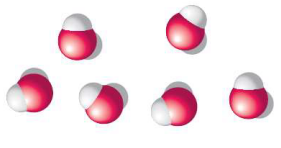
\includegraphics[width=.25\textwidth]{Composto molecolare.png}\\
                \fbox{
                    CH$_3$OH + CO \textrightarrow\ HCOOCH$_3$
                }
            \end{center}
        \end{figure*}
    \item I \textbf{composti ionici} sono costituiti da ioni positivi e negativi uniti da una forza
        di attrazione elettrica, nota come legame ionico:
        \begin{figure*}[h!]
            \begin{center}
                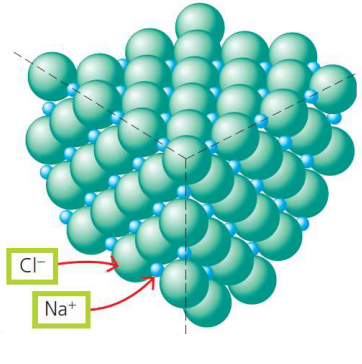
\includegraphics[width=.25\textwidth]{Composto ionico.png}\\
                \fbox{
                    \chemfig{\Charge{90=\.}{Na} + \Charge{90=\.,0=\|,-90=\|,180=\|}{Cl}} \textrightarrow\ 
                    \chemleft[\chemfig{Na}\chemright]$^+$\
                    \chemleft[\chemfig{\Charge{90=\|,0=\|,-90=\|,180=\|}{Cl}}\chemright]$^-$
                }
                
            \end{center}
        \end{figure*}
\end{itemize}

\subsection{Le equazioni chimiche}
Un'equazione chimica rappresentazione una reazione chimica mostrando come i reagenti si trasformano
in prodotti. Le formule chimiche dei reagenti e dei prodotti illustrano i rapporti numerici tra
le particelle coinvolte:
\begin{itemize}
    \item La freccia segnala la direzione in cui procede la reazione:
        \begin{itemize}
            \item da sinistra verso destra (\textrightarrow) i reagenti diventano prodotti;
            \item da destra verso sinistra (\textleftarrow) i prodotti tornano reagenti;
            \item in entrambe le direzioni ($\rightleftharpoons$) la reazione è reversibile.
        \end{itemize}
    \item Il simbolo presente sopra la freccia indica i processi o contributi al processo che
        avvengono durante la reazione chimica:
        \begin{itemize}
            \item \schemestart \arrow{->[$\Delta$][]} \schemestop
                indica il riscaldamento dei reagenti;
            \item \schemestart \arrow{->[$\uparrow$][]} \schemestop
                indica la liberazione di gas;
            \item \schemestart \arrow{->[$\downarrow$][]} \schemestop
                indica la formazione di precipitato.
        \end{itemize}
    \item Alcune annotazioni poste alla destra dell'atomo o della molecola indicano
        lo stato fisico dei reagenti e dei prodotti:
        \begin{itemize}
            \item X($g$): l'atomo o la molecola si trova in stato gassoso;
            \item X($s$): l'atomo o la molecola si trova in stato solido;
            \item X($l$): l'atomo o la molecola si trova in stato liquido;
            \item X($aq$): l'atomo o la molecola si trova in una soluzione acquosa.
        \end{itemize}
    \item I coefficienti stechiometrici posti davanti alle formule indicano la proporzione minima
        di molecole o ioni di ciascun reagente necessario per la reazione e di prodotti formati.
        Durante questo procedimento viene \textbf{\underline{bilanciata}} l'equazione chimica. 
        \begin{figure*}[h!]
            \begin{center}
                \fbox{\setchemfig{scheme debug=false}
                    \schemestart
                    C$_7$H$_{16}$($l$) + 11O$_2$($g$) \arrow{->[$\Delta$][]} 7CO$_2$($g$) + 8H$_2$O($g$)
                    \schemestop
                }
            \end{center}
        \end{figure*}
\end{itemize}
\pagebreak

\section{Mole e stechiometria}

\subsection{Massa atomica di un elemento}

La massa atomica di un elemento (\textit{MA}) è la media ponderata delle masse relative degli
isotopi presenti in un campione naturale
\hyperlink{massa atomica}{\color{blue}{(\underline{vedi 5.2})}}
\subsection{Massa molecolare}
La massa molecolare (\textit{MM}) si calcola sommando la massa atomica di tutti gli atomi che
formano il sistema:
\begin{figure*}[h!]
    \begin{center}
        \fbox{
            Molecola: $ApBqCr$\ \textrightarrow\ MM$_{ApBqCr}$ = p $\cdot$ MA$_A$ + q $\cdot$ MA$_B$ + r $\cdot$ MA$_C$
            
        }
    \end{center}
\end{figure*}
\subsection{La mole}
La mole è l'unità del Sistema Internazionale utilizzata per \textbf{quantificare il numero di
atomi o molecole in una data massa di sostanza}. È definita come la quantità di sostanza che
contiene tante entità elementari quanto il numero di Avogadro.
Utilizzando la mole, possiamo misurare e lavorare con quantità precise di sostanze a livello
atomico o molecolare.
\begin{figure*}[h!]
    \begin{center}
        \fbox{
            1 mol contiene 6.022 $\times  10^{23}$ particelle ($N_A$)
        }
    \end{center}
\end{figure*}
\subsection{Massa molare}
La massa molare (\textit{M$_{\text{mol}}$}) di una sostanza è numericamente uguale alla massa relativa (\textit{MA, MM})
di una sua particella.
\begin{figure*}[h!]
    \begin{center}
        \fbox{
            $M_{\text{mol}} [\frac{g}{\text{mol}}] = \frac{m [g]}{n_{\text{moli}}} [\text{mol}]$
        }
    \end{center}
\end{figure*}
\subsection{Volume molare}
Secondo il principio di Avogadro, a STP (temperatura e pressione standard: 0°C e 1atm),
volumi identici di gas diversi contengono lo stesso numero di particelle. Il volume molare è 
il \underline{volume occupato da una mole di qualsiasi gas} ed è lo stesso per tutti i gas nelle 
stesse condizioni di temperatura e pressione.
\begin{figure*}[h!]
    \begin{center}
        \fbox{
            Un gas, a STP, occupa un volume molare $V_{\text{mol}}=22.4\ \frac{L}{\text{mol}}$
        }
    \end{center}
\end{figure*}
\subsection{Molarità}
La molarità (\textit{M}) esprime la concentrazione di una soluzione.
Indica il numero di moli di soluto contenute in un litro di soluzione:
\begin{figure*}[h!]
    \begin{center}
        \fbox{
                $M = \frac{n}{V}\ [\frac{\text{mol}}{L}]$
            }\\
            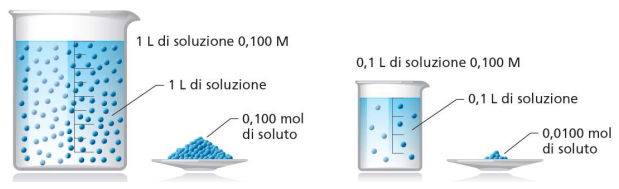
\includegraphics[width=.7\textwidth]{Molarità.png}
    \end{center}
\end{figure*}
\subsection{Reagente limitante}
Il reagente limitante è quello il cui esaurimento impedisce il proseguimento della reazione chimica,
il quale determina la massima quantità di prodotto che può essere formata. Se i rapporti
stechiometrici non sono perfettamente bilaciati, il reagente in eccesso rimarrà inutilizzato al
termine della reazione:
\begin{figure*}[h!]
    \begin{center}
        \fbox{
            3H$_2$ + O$_2$\ \textrightarrow\ 2H$_2$O + H
        }
    \end{center}
\end{figure*}\\
In questa reazione O$_2$ ne limita il proseguimento poiché è terminato, dunque:\\
O$_2$ è il reagente limitante, mentre H$_2$ è il reagente in eccesso.
\subsection{Resa di una reazione}
La resa di una reazione chimica si può classificare in tre categorie:
\begin{itemize}
    \item Resa teorica: è la quantità massima che si prevede di ottenere da una certa massa di
        reagente, calcolata secondo l'equazione bilanciata della reazione, espressa in moli;
    \item Resa effettiva: è la quantità reale di prodotto che si ottiene al termine della reazione,
        espressa in moli;
    \item Resa percentuale: è il rapporto percentuale tra la resa effettiva e la resa teorica.
\end{itemize}

\figbox{$\eta (\%) = \frac{\text{resa effettiva}}{\text{resa teorica}} \cdot 100$}

\pagebreak

\section{Legami chimici}

\subsection{Simbologia di Lewis}
La simbologia di Lewis è un metodo grafico per rappresentare la formazione dei legami chimici.
Questa notazione proietta gli elettroni del guscio più esterno, dunque quelli coinvolti nella
formazione dei legami, attraverso puntini disposti intorno al simbolo dell'elemento.
Una doppietta di elettroni non accoppiati possono essere indicati anche come una riga.
\figbox{
    \chemfig{\Charge{0=\.}{Li}} \quad
    \chemfig{\Charge{0=\.,180=\.}{Be}} \quad
    \chemfig{\Charge{0=\.,180=\.,90=\.}{B}} \quad
    \chemfig{\Charge{0=\.,180=\.,90=\.,-90=\.}{C}} \quad
    \chemfig{\Charge{0=\.,180=\.,90=\|,-90=\.}{N}} \quad
    \chemfig{\Charge{0=\.,180=\.,90=\|,-90=\|}{O}} \quad
    \chemfig{\Charge{0=\|,180=\.,90=\|,-90=\|}{F}} \quad
    \chemfig{\Charge{90=\|,0=\|,-90=\|,180=\|}{Ne}}
}
\subsubsection{Regola dell'ottetto}
La regola dell'ottetto afferma che gli atomi raggiungono stabilità massima quando possiedono
8 elettroni nel loro guscio esterno. Gli atomi tendono a perdere, guadagnare o condividere
elettroni fino a raggiungere questa conigurazione.
\figbox{\chemfig{\Charge{0=\.}{H} + \Charge{0=\|,180=\.,90=\|,-90=\|}{Cl}}\
    \textrightarrow\ \chemfig{H-\Charge{0=\|,90=\|,-90=\|}{Cl}}
}

\subsection{Legame ionico}
{\footnotesize Per la definizione di elettronegatività
\hyperlink{elettronegatività}{\color{blue}{\underline{vedi 4.7}}}.}\\
I composti ionici si originano dalla forza di attrazione elettrostatica tra ioni di segno opposto.
Durante la formazione di un composto ionico avviene un trasferimento di elettroni tra gli atomi coinvolti:
\begin{itemize}
    \item Un atomo cede uno o più elettroni e carica positivamente (catione);
    \item L'altro atomo prende gli elettroni ceduti e si carica negativamente (anione).
\end{itemize}
\figbox{
    \begin{minipage}{.85\textwidth}
        Il trasferimento di elettroni avviene quando la differenza assoluta di elettronegatività
        ($|\Delta E_N|$) tra due atomi è maggiore di 1.7
    \end{minipage}
}
Se per esempio si facesse reagire del sodio e del cloro si formerebbe un composto ionico:
\figbox{
    \begin{minipage}{.4\textwidth}
        \centering $\Delta E_N$ = 3.16 (Cl) - 0.93 (Na) = 2.21\\ \phantom{} \\
        \chemfig{\Charge{90=\.}{Na} + \Charge{90=\.,0=\|,-90=\|,180=\|}{Cl}} \textrightarrow\ 
        \chemleft[\chemfig{Na}\chemright]$^+$\
        \chemleft[\chemfig{\Charge{90=\|,0=\|,-90=\|,180=\|}{Cl}}\chemright]$^-$
    \end{minipage}
}

\subsection{Legame covalente}

Il legame covalente si forma attraverso la condivisione di elettroni tra due atomi. Durante la
formazione di una molecola, gli elettroni vengono attratti da entrambi i nuclei.
Con il diminuire della distanza tra nucleo e nucleo, aumenterà la densità elettronica probabile
nello spazio.
\figbox{\parbox{\textwidth}
    {Il legame covalente può essere di due tipi:
        \begin{itemize}
            \item \textbf{Legame covalente puro}: si forma tra atomi con $|\Delta E_N|$ compreso tra 0 
                (due atomi uguali) e 0.45;
            \item \textbf{Legame covalente polare}: si forma tra atomi con $|\Delta E_N|$ tra 0.45 
                e 1.7 non compresi.
        \end{itemize}
    }
}\\
Se si facessero reagire due atomi di ossigeno con uno di carbonio si otterrebbe un legame
covalente polare:
\figbox{
    \begin{minipage}{.4\textwidth}
        \centering $\Delta E_N$ = 3.44 (O) - 2.55 (C) = 0.89\\ \phantom{} \\
        \chemfig{\Charge{135=\|,-135=\|}{O}=C=\Charge{45=\|,-45=\|}{O}}
    \end{minipage}
}

\subsection{Valori di legame}
\phantom{}
\begin{center}
    \begin{tikzpicture}
        \draw[thick, -] (0,0) -- (15,0);
        \draw (0 cm, 5pt) -- (0 cm, -3pt);
        \draw (5 cm, 5pt) -- (5 cm, -3pt);
        \draw (10 cm, 5pt) -- (10 cm, -3pt);
        \draw (15 cm, 5pt) -- (15 cm, -3pt);
    
        \node at (0, 0.5) {0};
        \node at (5, 0.5) {0.45};
        \node at (10, 0.5) {1.7};
        \node at (2.5, -0.3) {Legame covalente puro};
        \node at (7.5, -0.3) {Legame covalente polare};
        \node at (12.5, -0.3) {Legame ionico};
    \end{tikzpicture}
\end{center}
\phantom{} 

\subsection{Energia potenziale}
L'energia potenziale di una molecola varia in base alla distanza tra i nuclei atomici.
L'energia, a causa delle forze di repulsione, aumenta quando i nuclei sono eccessivamente vicini,
mentre raggiunge il minimo quando si trovano a una distanza ottimale l'uno dall'altro.
Quando l'energia potenziale è minima, allora la molecola è nella sua configurazione più stabile.
\begin{figure*}[h!]
\centering 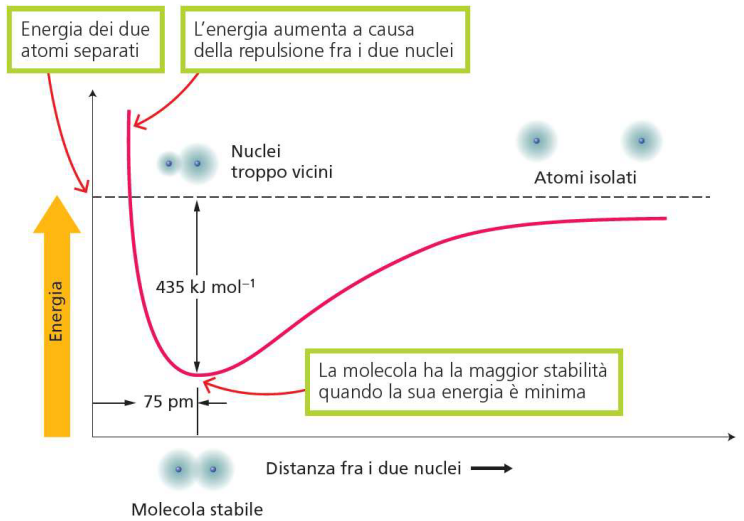
\includegraphics[width=.8\textwidth]{grafico legame covalente.png}
\end{figure*}\\
Da questo grafico si enuncia che idealmente la reazione chimica tra due atomi avvenga quando 
i loro nuclei si trovano alla distanza ideale e che questo processo sia esotermico (libera energia).

\subsection{Numero di ossidazione}
Il numero di ossidazione (N.O) rappresenta la carica formale che si può attribuire a un elemento
in un composto, supponendo che tutti i legami siano di tipo ionico, in modo da assegnare gli
elettroni di legame all'elemento più elettronegativo.
\figbox{\parbox{\textwidth}
    {\begin{itemize}
        \item N.O $<$ 0\ \textrightarrow\ Ione negativo oppure l'atomo ruba l'elettrone a un atomo meno
            elettronegativo;
        \item N.O = 0\ \textrightarrow\ L'atomo non ha legami oppure il legame ha una forza
            intramolecolare $|\Delta E_N|=0$;
        \item N.O $>$ 0\ \textrightarrow\ Ione positivo oppure l'atomo cede l'elettrone a un atomo più
            elettronegativo.
    \end{itemize}}
}
\pagebreak

\subsection{Carica formale}
La carica formale (FC) è un concetto usato per descrivere la carica elettrica di un atomo
all'interno di una molecola, basandosi sull'ipotesi che gli elettroni di legame siano distribuiti
equamente tra gli atomi, indipendemente dalla loro elettronegatività.
\figbox{
    $FC = N-(\overline{C}+\frac{C}{2})$
}\\
dove:
\begin{itemize}
    \item $N$ = numero di elettroni di valenza dell'atomo neutro;
    \item $\overline{C}$ = numero di elettroni di valenza non condivisi;
    \item $C$ = numero di elettroni di legame condivisi.
\end{itemize}

\subsection{Formula di struttura semplificata}
Le strutture delle molecole organiche {\color{red}METTERE HYPERLINK ORGANICA} possono essere scritte
nella loro formula semplificata:
\figbox{
    \chemfig{H-C(-[:90]H)(-[:-90]H)-C(-[:90]H)(-[:-90]H)-C(-[:90]H)(-[:-90]H)-O-H}\
    \textrightarrow\ CH$_3$CH$_2$CH$_2$OH\ \textrightarrow\
    \chemfig{-[:45]-[:-45]-[:45]OH}
}



\pagebreak

\section{Geometria molecolare VSEPR}
La geometria di una molecola può essere rappresentata ricorrendo al modello VSEPR
(Valence Shell Electron Pair Repulsion), il quale principio è basato sulla repulsione degli
elettroni di valenza, i quali tendono a collocarsi alla maggior distanza possibile l'uno
dall'altro.
\vspace*{1.9cm}

\begin{center}
    \fbox{
        \makecell[l]{ 
            \hspace*{.5cm}Geometria
            \hspace*{1.65cm}
            Prospettiva
            \hspace*{1.05cm}
            Modello a sfere \\ \\
            Geometria lineare: \qquad
            \chemfig{
                \Charge{90=\|,-90=\|}{O}=C=\Charge{90=\|,-90=\|}{O}
            } \qquad
            \chemfig{
                @{1}\circled{O}=@{2}\circled{C}=@{3}\circled{O}
            } \arclabel{-0.5cm}{1}{2}{3}{\footnotesize180\textdegree}{-90}{-8.5pt} \\ \\ \\
            Triangolare planare:
            \hspace*{.175cm}
            \chemleft[
                \chemfig{
                    {\Charge{90=\|,-180=\|}{O}}
                    =[:-45]C(-[:-90]{\Charge{0=\|,-90=\|,-180=\|}{O}})
                    -[:45]\Charge{45=\|,135=\|,-45=\|}{O}
                } 
            \chemright]$^{2-}$
            \hspace*{.35cm}
            \chemfig{
                @{0}\circled{O}
                -[:-45]@{1}\circled{C}(-[:-90]@{2}\circled{O})
                =[:45]@{3}\circled{O}
            } \arclabel{0.5cm}{0}{1}{2}{\footnotesize120\textdegree}{-202.5}{0} \\ \\ \\
            Tetraedrica:
            \hspace*{1.85cm}
            \chemfig{
                H-[:-90]C(<:[:-135]H)(<[:-90]H)(-[:-45]H)
            }
            \hspace*{1cm}
            \chemfig{
                @{0}\circled{H}-[:-90]@{1}\circled{C}(-[:-165]@{2}\circled{H})(-[:-90]\circled{H})(-[:-15]\circled{H})
            } \arclabel{.6cm}{0}{1}{2}{\footnotesize107.3\textdegree}{-142.5}{2pt} \\ \\ \\
            Piramidale triangolare:
            \hspace*{.16cm}
            \chemfig{
                \Charge{90=\|}{N}(<:[:-135]H)(<[:-90]H)(-[:-45]H)
            }
            \hspace*{1cm}
            \chemfig{
                @{0}\circled{N}(-[:-165]\circled{H})(-[:-90]@{1}\circled{H})(-[:-15]@{2}\circled{H})
            } \arclabel{.7cm}{1}{0}{2}{\footnotesize109\textdegree}{-270}{.5} \\ \\ \\
            Piegata:
            \hspace*{2.4cm}
            \chemfig{
                \Charge{45=\|,135=\|}{O}(-[:-45]H)(-[:-135]H)
            }
            \hspace*{1.15cm}
            \chemfig{
                @{1}\circled{O}(-[:-30]@{2}\circled{H})(-[:-150]@{0}\circled{H})
            } \arclabel{.6cm}{0}{1}{2}{\footnotesize104.5\textdegree}{-270}{.5} \\ \\ \\
            Bipiramidale trigonale:
            \hspace*{.075cm}
            \chemfig{
                Cl-[:-90]P(-Cl)(-[:-90]Cl)(<[:-135]Cl)(<:[:135]Cl)
            }
            \hspace*{.95cm}
            \chemfig{
                @{3}\circled{Cl}-[:-90]@{1}\circled{P}(-@{4}\circled{Cl})(-[:-90]\circled{Cl})
                (-[:-135]@{0}\circled{Cl})(-[:135]@{2}\circled{Cl})
            }
            \arclabel{.5cm}{0}{1}{2}{\footnotesize120\textdegree}{-180}{.5} 
            \arclabel{.6cm}{3}{1}{4}{\footnotesize90\textdegree}{-45}{2} \\ \\ \\
            Ottaedrica:
            \hspace*{1.75cm}
            \chemfig{
                F-[:-90]S(-[:-90]F)(<:[:30]F)(<:[:150]F)(<[:-150]F)(<[:-30]F)
            }
            \hspace*{1.05cm}
            \chemfig{
                \circled{F}-[:-90]@{1}\circled{S}(-[:-90]@{0}\circled{F})(-[:30]\circled{F})(-[:150]\circled{F})
                (-[:-150]\circled{F})(-[:-30]@{2}\circled{F})
            }
            \arclabel{.6cm}{0}{1}{2}{\footnotesize90\textdegree}{-299}{1} \\
            \phantom{}
        }
    }
\end{center}
\pagebreak

\section{Termochimica}
TODO
\pagebreak

\section{Cinetica}
TODO
\pagebreak

\section{Equilibrio chimico}
TODO
\pagebreak

\section{Reazioni di ossidoriduzione}
TODO
\pagebreak

\section{Equilibrio acido base}
TODO
\pagebreak

\section{Chimica organica}
TODO




\end{document}
